\documentclass[11pt, oneside]{article}    % use "amsart" instead of "article" for AMSLaTeX format
\usepackage{geometry}                   % See geometry.pdf to learn the layout options. There are lots.
\usepackage{acl2014} 
\geometry{letterpaper}                      % ... or a4paper or a5paper or ... 
%\geometry{landscape}                   % Activate for for rotated page geometry
% \usepackage[parfill]{parskip}       % Activate to begin paragraphs with an empty line rather than an indent
\usepackage{graphicx}       % Use pdf, png, jpg, or eps§ with pdflatex; use eps in DVI mode
                % TeX will automatically convert eps --> pdf in pdflatex    
\usepackage{amssymb}
\bibliographystyle{acl}
%\usepackage{cite}
\usepackage{amsmath}
\usepackage{multirow}
\usepackage{tabularx}

% Zifei: seems that most ACL papers use times font which is more compact
\usepackage{times}
\usepackage{url}
\usepackage{latexsym}


\title{Authorship Attribution in Multi-author Documents}

\author{Tim Althoff, Denny Britz, Zifei Shan \\
  Department of Computer Science, Stanford University \\
  {\tt \{althoff, dbritz, zifei\}@cs.stanford.edu} \\
  }
  
% \author{ Tim Althoff \\
%   {\tt althoff@cs.stanford} \\\And
%   Denny Britz \\
%   {\tt dbritz@cs.stanford} \\\And
%   Zifei Shan \\
%   {\tt zifei@cs.stanford} \\
% }

% \author{ Tim Althoff, Denny Britz, and Zifei Shan \\
%   {\tt \{althoff, dbritz, zifei\}@cs.stanford.edu} \\
% }

\begin{document}
\maketitle

\begin{abstract}

Authorship attribution, the task of identifying the author of a document, has been applied to works of historical value such as Shakespeare's plays or the political Federalist papers but is still highly significant in identifying users across online communities, detecting impersonation attacks, or ensuring anonymity in double-blind conference submission processes.
We introduce the novel problem of authorship attribution in multi-authored documents and focus on scientific publications.
We demonstrate using a stylometric approach that paper authors can be predicted with significant accuracy by exploiting authors' stylistic idiosyncrasies.
This challenges the assumption that simply removing names from a paper submission ensures anonymity in a double-blind process.
Multi-authored documents present hard challenges for authorship attribution.
We propose several ideas how these can be addressed and evaluate when such models perform well.
To this end we present a sentence-based prediction model that also allows to estimate which sentences were contributed by which author.

\end{abstract}

\section{Introduction}\label{sec:intro}
% !TEX root = cs224_final_paper.tex

Authorship attribution, the science of identifying the rightful author of a document,
is a problem of long-standing history.
The main idea behind statistically or computationally supported authorship attribution is that by measuring some textual features, we can distinguish between texts written by different authors.
The pioneering study of Mendenhall \cite{mendenhall1887characteristic} in the 19th century marks the first attempt to quantify writing style on the plays of Shakespeare.
In the first half of the 20th century it was followed by statistical studies by Yule \cite{yule1939sentence,yule1944statistical} and Zipf \cite{zipf1932selected}. 
Later in 1964, the study by Mosteller and Wallace \cite{mosteller1964inference} on the authorship of ``The Federalist Papers'' (a series of 146 political essays written by John Jay, Alexander Hamilton, and James Madison, 12 of which claimed by both Hamilton and Madison) is considered the most influential work in authorship attribution \cite{stamatatos2009survey}. 
% Historical successes included the confirmation of the collaboration of Shakespeare with his contemporaries Fletcher and Christopher Marlowe \cite{matthews1993neural,merriam1994neural}  as well as the
% resolution of disputed authorship in twelve of the Federalist Papers by Frederick Mosteller and David Wallace \cite{mosteller1964inference}.

Identifying the author of a document also has modern applications such as identifying and linking users across online communities or detecting fraudulent transactions and impersonation attacks.

Thus far, work has focused on predicting authors of single-authored documents such as plays \cite{mendenhall1887characteristic,matthews1993neural,merriam1994neural}, political essays \cite{mosteller1964inference}, or blog posts \cite{narayanan2012feasibility}.
In contrast, this paper introduces the problem of authorship attribution in multi-authored documents such as academic research papers.
To the best of our knowledge, this problem has never been tackled before.

However, this problem is important. 
For instance, many computer science conferences employ a double-blind submission process, relying on the assumption that identifying the authors of submitted papers based on content and style is impossible or at least highly impractical. 
We challenge this notion by presenting an stylometric approach that is able to identify the authors of anonymous papers with significant accuracy by exploiting authors' stylistic idiosyncrasies.

Identifying the authors of multi-authored documents presents new challenges.
Since it is unclear which author contributed which part of a document, we lack ground truth that could be used to build a model for each author.
Employing a document-level perspective as done in previous work confuses idiosyncrasies of several authors leading to problems during classification (see section \ref{subsec:author_mixing}).
We propose employing a sentence-level perspective in which we predict an author for each individual sentence and then aggregate those to paper-level author predictions as a more sensible strategy for multi-authored publications. 

The rest of the paper is organized as follows: Section \ref{sec:related_work} discussed related work, section \ref{sec:approach} presents a formal definition of our proposed model, section \ref{sec:experiments} presents features and datasets and section \ref{sec:results} discussed experimental results. 

\section{Related Work}\label{sec:related_work}
% !TEX root = cs224_final_paper.tex

A large body of research exists on attributing authorship on the document level. 
Approaches can broadly be categorized into varying among the dimensions of feature selection, model selection, and candidate selection ~\cite{stamatatos2009survey}. 
Features can be divided into lexical (token- and word features), character (character n-grams), syntactic (POS tags, phrase structure), semantic (synonymous and dependencies) and application-specific features \cite{stamatatos2009survey}. 
More sophisticated features such as local histograms~\cite{escalante2011local} and grammatical errors ~\cite{koppel2003exploiting} have also been explored. 
Authorship attribution approaches taking into account only self-citations often perform well ~\cite{hill2003myth} compared to their supervised counterparts. 

Overall, the choice of model seems to have a smaller impact than the choice of features, and a variety of supervised and unsupervised Machine Learning methods have been applied to the problem of authorship attribution~\cite{stamatatos2009survey}. 
Simple similarity-based models (nearest-neighbors) also perform surprisingly well ~\cite{koppel2012fundamental} and often outperform more ``sophisticated'' supervised classifiers such as SVMs. 
One of the reasons behind this is an issue known as ``masking''~\cite{narayanan2012feasibility}. The size of the candidate author set is another important dimension. Sets of hundreds of candidate authors seems most common. Once the set of candidate authors get significantly larger the problem becomes more challenging. Only few researchers have applied attribution models to web-scale data ~\cite{narayanan2012feasibility}. 

Predicting authors in multi-authored scientific publications has been out of focus of the scientific community thus far (to be best of our knowledge).
However, some work has looked at using scientific publications to predict gender~\cite{sarawgi2011gender,bergsma2012stylometric} and whether or not the publication was written by a native speaker or submitted to a workshop instead of a conference~\cite{bergsma2012stylometric}.




\section{Approach}\label{sec:approach}
% !TEX root = cs224_final_paper.tex

\subsection{Author mixing}\label{subsec:author_mixing}

TODO: Explain the issue with having different authors and put picture here.

\subsection{Notation}

Our corpus $(P,A)$ consists of a set of papers $P=\{p_1, \dots, p_N\}$ and a set of authors $A=\{a_1, \dots, a_K\}$.
Each paper $p_i$ is divided into sentences $s_j^i \in p_i$ that we assume were written by a single author $\mathtt{author_s}(s_j^i)=a_k$.
Alternatively, we could model one author per paragraph or section but it is less clear that such assumptions would hold in practice.
While we assume that a sentence is written by a single author we do not actually observe author labels on sentence level.
We only observe paper level authors and assume that the sentence author is one of the paper authors.
Mathematically, given paper level annotation $\mathtt{author_p}(p_i)=\{a_1, a_7, a_9\}$ we assume 
$$\forall s_j^i\in p_i: \mathtt{author_s}(s_j^i) \in \mathtt{author_p}(p_i)$$

Our goal is to learn to differentiate author styles from the ambiguous ground truth labels $\mathtt{author_p}$ such that we can assign each sentence in a paper to a single author.

We represent this mapping from sentence to author as a matrix $M$ that, for all sentences, contains the single author that is believed to have written that sentence, e.g. $M(s_j^i)=a_k$.
The authors' individual styles are captured through parameters $\theta=(\theta_1, \dots, \theta_K)$ that includes an independent parameter vector for each author $a_k \in A$.

\subsection{Sentence authorship model}
The core of our model describes how likely a given author $a$ is to have generated a given sentence $s$, $p(a|s)$.
We represent a sentence through features $F(s) \in \mathcal{R}^n$ (for more details on our features please refer to section \ref{sec:features}).
We use the following logit model:
\begin{align*}
p(a|s) &=& \operatorname{logit}^{-1}(\langle\theta_a, F(s)\rangle) \\
&=& \frac{1}{1+ \exp({-\langle\theta_a, F(s)\rangle}})
\end{align*}


Note that this model formulation is equivalent to a log-linear model:
$$\log p(\mathtt{author_s}(s)=a | s) = \langle\theta_a, F(s)\rangle - \log Z$$
where $Z$ is a normalizing constant 
$$Z= 1 + \exp(\langle\theta_a, F(s)\rangle).$$

Further note that we have $K$ of these models, one for each author.


\subsection{Learning to differentiate author styles from ambiguous labels}
\label{subsec:fancy_training}

\begin{figure*}[htbp]
\begin{center}
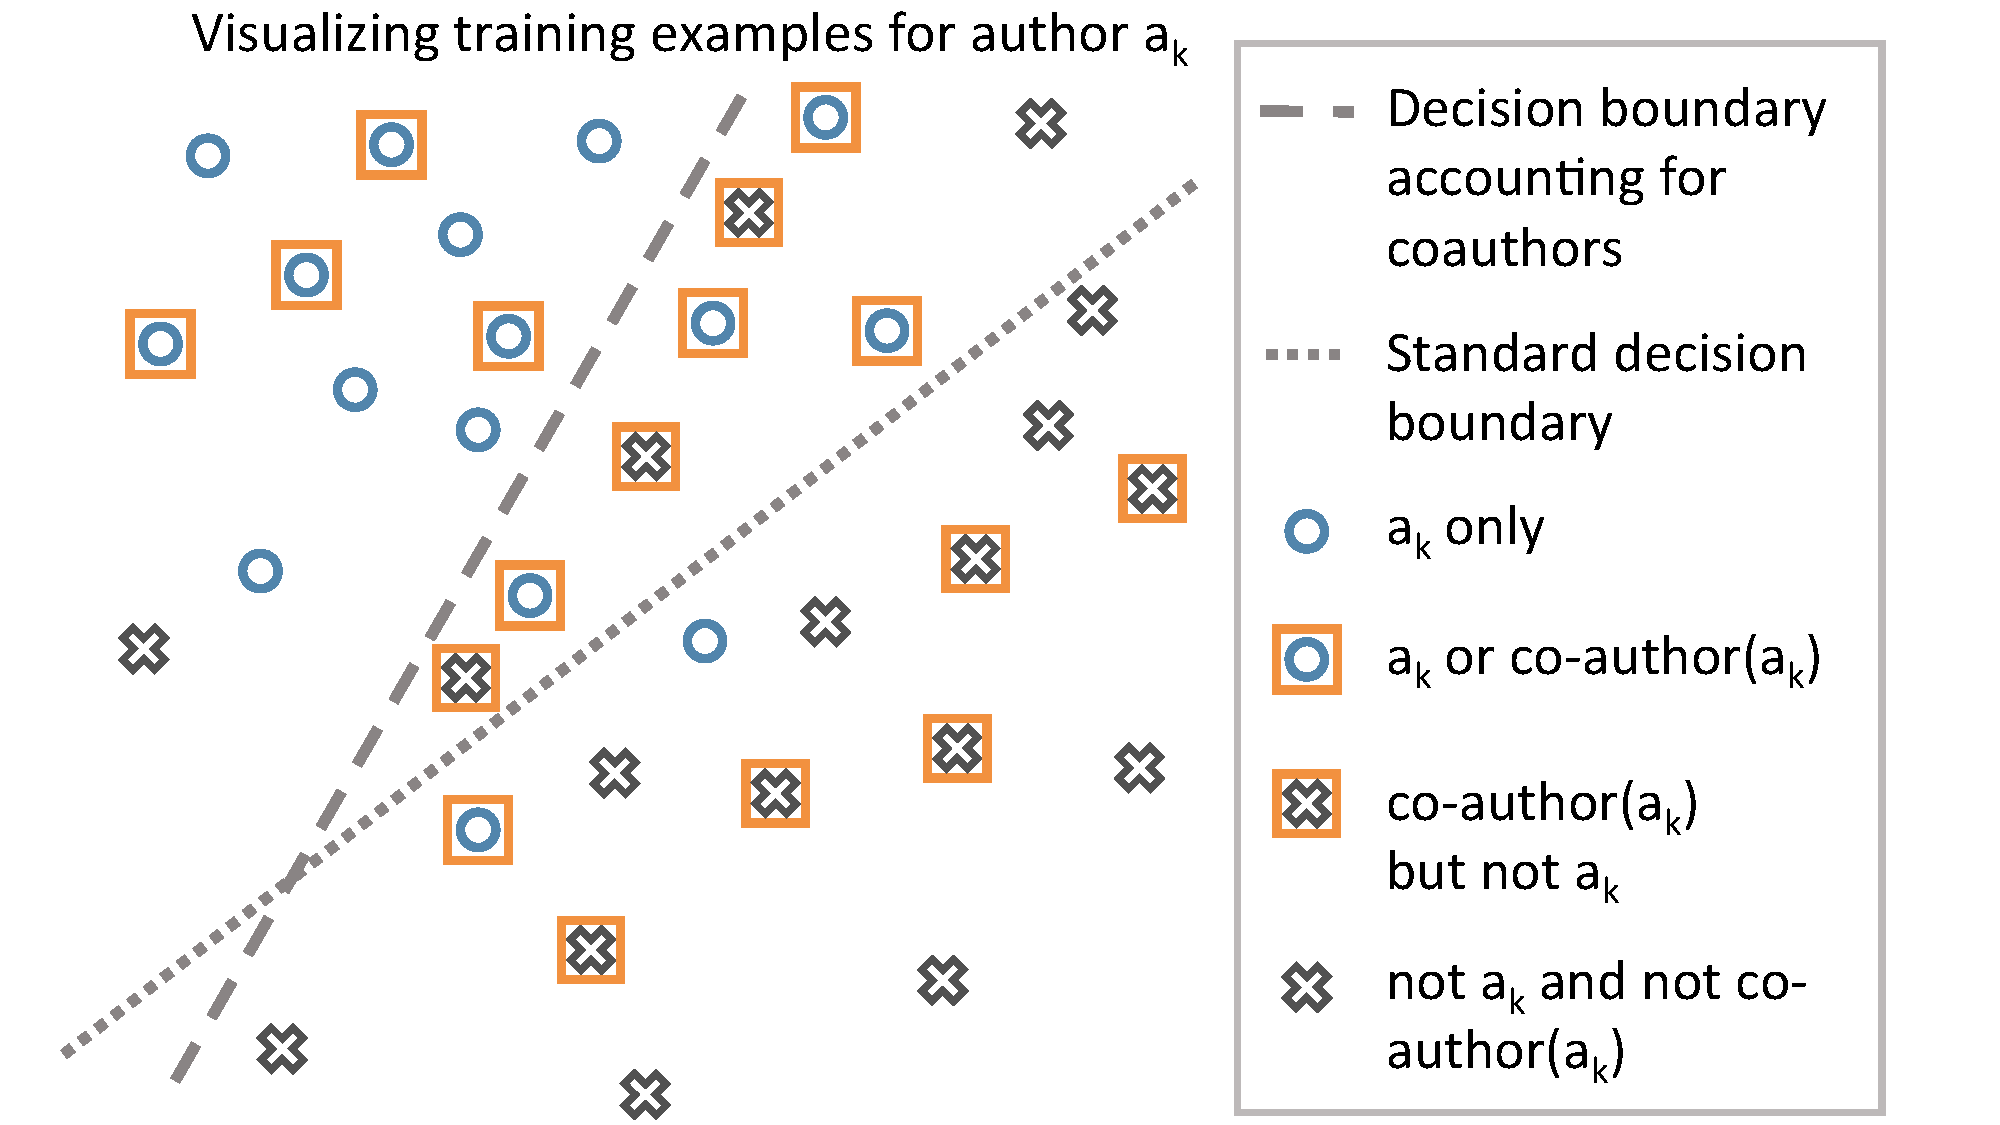
\includegraphics[width=\linewidth]{fancy_training.pdf}
\caption{Training procedure considering co-author negative examples in addition to random negative examples}
\label{fig:fancy_training}
\end{center}
\end{figure*}


A core challenge in learning such logit models is that we lack sentence-level author labels.
As described above, we only observe paper level author labels, i.e. $\mathtt{author_s}(s_j^i) \in \mathtt{author_p}(p_i)$ but we have no basis for assuming any concrete author yet.

Let the authors of a paper $p_i$ be $\mathtt{author_p}(p_i) = \{ a_1, a_2\}$.
To train a model for author $a_1$ we need both positive examples (sentences that $a_1$ did write) and negative example (sentences that $a_1$ did not write). 
For any sentence $s_j^i \in p_i$ we do not know whether it was written by $a_1$ or $a_2$, i.e. we have ambigious sentence labels.
Negative examples are much easier to come by, sentences from any paper that $a_1$ did not co-author would provide true negative examples.

Since we have no basis for assuming, a priori, that sentence $s_j^i$ was definitly written by either $a_1$ or $a_2$ we include all sentences that $a_1$ might have written as positive examples when training an author model for $a_1$. 
Obviously, this will include false positive examples that $a_2$ actually wrote and we need to make sure that we train a model that captures $a_1$'s style and not the combined style of $a_1$ and $a_2$.
To this end, we propose to carefully select negative examples that differentiate $a_1$'s style from the one of $a_2$.
We can achieve this by including positive examples from $a_2$ in as negative examples for $a_1$ (only those sentences that $a_1$ certainly did not write).
In fact, we do not only include but positive examples from all co-authors of $a_1$.
This idea is visualized in Figure \ref{fig:fancy_training}.

In the following, we describe this idea more formally.
We denote the set of all coauthors of a given author $a_k$ by 
\begin{align*}
\mathtt{coauthor}(a_k) =  \{ &a_l \in A \;|\; \forall p\in P: \\
a_l \in \mathtt{author_p}(p) & \Rightarrow a_k \in author_p(p) \}
\end{align*}

Formally, we use the following set of positive examples for $a_k$:
$$ \mathtt{POS}(a_k) = \{ s_j^i \in p_i \;|\; a_k \in \mathtt{author_p}(p_i)\}$$

And the following set of negative examples for $a_k$:
\begin{align*}
\mathtt{NEG}(a_k) = \{ s_j^i \in p_i \;|\; \exists  a_l \in \mathtt{coauthor}(a_k): \\
 a_l \in \mathtt{author_p}(p_i) \wedge a_k \notin \mathtt{author_p}(p_i) \}
\end{align*}

We further add random sentences to $\mathtt{NEG}(a_k)$ since authors have a varying number of co-authors and those with few would end up with very few negative examples otherwise.
%This way of training will be contrasted to just using random negative examples in Section TODO.

\subsection{Refining author models through Expectation Maximization}
Modeling authorship on sentence level gives us the opportunity to further refine our author models (this is not possible on paper level).
The approach described above uses all sentences that could possibly have been written by author $a_k$ as positive examples (recall $\mathtt{POS}(a_k)$).
However, this will include many sentences that were actually written by  one of $a_k$'s coauthors.
Based on our confidence about which sentences were likely written by $a_k$ we can filter the positive examples to yield a cleaner set of positive examples for $a_k$.
We now formalize this intuion.

For the likelihood of the full corpus $(P,A)$ we treat each sentence independently:
$$P(M,\theta | P,A) = \prod_{p_i \in P} \prod_{s_j^i \in p_i} p(M(s_j^i) | s_j^i).$$

The parameter inference problem then becomes
$$\hat{M},\hat{\theta} = \operatorname{argmax}_{M,\theta} P(M,\theta | P,A) - \Omega(M,\theta),$$
where $\Omega(M,\theta)$ is a regularizer on the parameters to avoid overfitting.

Since this optimization depends on both $M$ and $\theta$ we proceed by coordinate ascent on $(M, \theta)$, i.e. by alternately optimizing
$$M^i = \operatorname{argmax}_{M} P(M,\theta^i|A,P)$$
and
$$\theta^{i+1} = \operatorname{argmax}_{\theta} P(M^i,\theta|A,P)$$
until convergence, i.e. until $M^i$ differs from $M^{i-1}$ on less than a prespecified number of sentences (alternatively, one can alternate for a constant number of iterations).

Being a local optimization procedure, coordinate ascent is sensitive to initialization.
Therefore, we initialize the style parameters for each author $\theta^{0}$ by training independent logistic regression models using all sentences an author could have possibly written as positive examples and sentences by his co-authors that he could not have written as well as random other sentences by other authors as negative examples (as formally described in Section \ref{subsec:fancy_training}).

Optimizing for $M$ then is a simple inference step where we dependently assign each sentence to the most likely possible author:
$$M(s_j^i) = \operatorname{argmax}_{a} p(a|s_j^i, \theta)$$

Based on this assignment, optimizing for $\theta$ then becomes estimating $K$ independent logistic regression models for all authors based on the assignment $M$.


\subsection{Predicting paper authors from sentence authors}
Our proposed model gives us predictions on sentence-level $M(s_j^i)$.
While those sentence-level predictions are interesting in its own right (e.g. to estimate contribution of different authors) we ultimately want to predict authors on paper-level.
To this end, we aggregate our sentence-level predictions to paper level predictions by having each sentence $s_j^i$ vote for its most likely author (namely, $M(s_j^i)$).

Compared to this hard voting scheme we also experimented with a soft voting scheme where each author gets a fractional vote depending on their confidence to have written this particular sentence.
However, empirically we found that soft-voting across all sentences of a paper suffers from the same problems that paper-level predictions do \ref{subsec:author_mixing}. 
Hard voting performed better in all test cases.

\section{Experimental Setup}\label{sec:experiments}
% !TEX root = cs224_final_paper.tex

\begin{table}[t]
\begin{center}
\begin{tabular}{c p{1.5cm} p{2.5cm}}
 \hline
& \textbf{Synthetic dataset} & \textbf{Real-world dataset} \\ \hline
Authors & 108 & 100 \\
Publications & 360 & 234 \\
Sentences & 78,577 & 206,300 \\
 \hline
\end{tabular}
\end{center}
\caption{Descriptive statistics of the datasets}
\label{table:data}
\end{table}%

We evaluate our hypothesis on both synthetic and realistic data. We obtained scientific publications available through arXiv. The complete set of PDF documents includes about 700,000 publications. We converted all PDF documents into raw text files using Apache Tika\footnote{http://tika.apache.org/}. For documents in either one of the two datasets we produced sentence tokenizations, POS annotations and dependencies parses using Stanford CoreNLP\footnote{http://nlp.stanford.edu/software/corenlp.shtml} on the converted text files. The datasets are summarized in table \ref{table:data}.

\subsection{Synthetic Data}

In order to evaluate our sentence-level predictions we generated an synthetic dataset with sentence-level labels as follows. Let $A$ be the set of authors such that every author $a \in A$ has more than 10 single-authored papers and more than 120 paragraphs with at least 500 words. Let $P_a$ be the set of paragraphs of more than 500 words written by $a \in A$. We generate a document by randomly picking 3 authors $a_1, a_2, a_3 \in A$ and sampling 40 paragraphs from $P_{a_1}, P_{a_2}, P_{a_3}$ without replacement. We repeat this procedure until not enough paragraphs are left to generate a full document. This procedure yields a corpus of 108 authors, 360 publications, 14,027 paragraphs and 78,577 sentences.  Each author gets approximately the same number of publications and paragraphs.

\subsection{Real-world Data}

To test our model in the real world, we subsample the arXiv dataset. We are interested in distinguishing authors in similar fields, therefore we start from a list of authors (``bootstrap list'') working in the field of social and information networks.
\footnote{These authors include: Alex Pentland, Bernardo Huberman, Brian Karrer, Johan Ugander, Jon Kleinberg, Jure Leskovec, Lada Adamic, and Lars Backstrom. (sorted by first name)} 
% We selected all papers written by any of these authors, resulting in a corpus of 150 papers, 169 authors (the 8 authors in the ``bootstrap list'' and their 161 coauthors), 91,036 paragraphs and 183,437 sentences. We note that this dataset is highly imbalanced. The 8 bootstrapped authors have a large amount of training data while their co-authors have relatively little training data.
We sample a set of papers written by any of these authors and their coauthors, controlling each author to have at most 10 papers. We get a corpus of 234 papers, 100 authors (the 8 authors in the ``bootstrap list'' and their 92 coauthors) and 206,300 sentences.


\subsection{Features}\label{sec:features}

The parameters of our models correspond to features categorized into content and style. Table \ref{table:features} contains a detailed description of the feature space we are considering. Some design decisions in our features include:

(1) We try to find a clear boundary between stylistic features and content features. While character unigrams can be regarded as purely stylistic, we found that character N-grams can reveal content (e.g. ``NCP''). Therefore we treat character N-grams as a content feature while unigrams as a stylistic feature.

(2) Among stylistic features, \textit{function words} are defined as
all words other than nouns, verbs, adjectives, and adverbs (which are
regarded as ``content words''), indicated by their POS tags. In
function word features, numbers are unified into a placeholder
\texttt{-NUMBER-} to hide content and reduce sparcity.

\begin{table*}[t]
\begin{center}
\small
\bgroup
\def\arraystretch{1.5}
\begin{tabular}{l p{3.5cm} p{5cm} p{4cm}}
 \hline
\textbf{Type} & \textbf{Feature Name} & \textbf{Description} & \textbf{Examples} \\ 
\hline
Content   & Word N-grams       & Unigrams, bigrams, and trigrams of all words.        & ``a distance matrix'', ``quartet topologies embedded''   \\
          & Character N-grams  & Bigrams and trigrams of characters.                  & ``NWD'', ``Ref''                  \\
\hline
Stylistic & Character unigrams & Unigrams of characters.                             & `\%', `\{', `?', `$\alpha$'                           \\
          & POS tag N-grams    & Unigrams and bigrams of POS tags (tagged by NLTK default Penn Treebank POS tagger). &  DT NN, PRP VBP, -LRB- NN \\
          & Function word N-grams & unigrams, bigrams, and trigrams of function words.  & ``under our'', ``but all the''    \\
          & Lengths            & Sentence length and average word length of each sentence. & 81 chars, 17 words, average word length=4.7 \\
          & Sentence start     & First word in sentence if it is a function word.    & ``We'', ``It'', ``However''       \\
          & Transition words   & First word after a punctuation if it is a function word. & ``However, we observe'' would give the feature ``we''.\\
          & Punctuation sequence & Concatenation of all the punctuations in a sentence. & ``.'', ``,.'', ``,;,.'', ``,().'' \\
          & Sentence shape     & Punctuation sequence and number of words (``M'' if more than 3) between each two punctuations. & ``3,M;2,M.'' \\
\hline
\end{tabular}
\egroup
\end{center}
\caption{Features}
\label{table:features}
\end{table*}


%
%\subsection{Content features}
%
%We use the following features that captures the content:
%
%
%\begin{itemize}
%\small
%\item
%  \textbf{Word N-grams} (unigrams, bigrams, and trigrams)
%\item
%  \textbf{Character bigrams and trigrams}
%\end{itemize}
%
%\subsection{Stylistic Features}
%
%We design the following stylistic features:
%
%\begin{itemize}
%\small
%\item
%  \textbf{Character unigrams}
%\item
%  \textbf{POS tag N-grams} (unigrams and bigrams). We used NLTK default POS tagger (Penn Treebank) to obtain POS tags.
%\item
%  \textbf{Function word N-grams} (unigram, bigram, trigram). Function
%  words are defined as all words other than nouns, verbs, adjectives,
%  and adverbs (which are regarded as ``content words''), indicated by
%  their POS tags. In function word features, Numbers are unified into a
%  placeholder \texttt{-NUMBER-} to hide content and reduce sparcity.
%\item
%  \textbf{Sentence length} and \textbf{average word length} for each sentence.
%\item
%  \textbf{Sentence start}: we capture how a sentence is started by its
%  first word if it is a function word. (e.g. ``We'', ``It'',
%  ``However'')
%\item
%  \textbf{Transition words}: we capture how transitions are made by
%  every first word after a punctuation if it is a function word. (e.g.
%  ``However, we observe'' would give the feature ``we'')
%\item
%  \textbf{Punctuation sequence}: we concatenate all the punctuations in a
%  sentence as a feature to capture punctuation habits in sentences.
%  (e.g. ``,,,,.'' or ``,;,.'')
%\item
%  \textbf{Sentence shape}: we capture sentence shape by punctuations and
%  the number of words between each two of them. If there are more than 3
%  words between two punctuations, we mark it as ``many''. (e.g.
%  ``3,M;2,M.'')
%\end{itemize}


\section{Results}\label{sec:results}
% !TEX root = cs224_final_paper.tex

\begin{table*}[htdp!]
\begin{center}
\begin{tabular}{|c|c|c|c|c|}
\hline
& LR (synthetic) & EM (synthetic)  & LR (real-world) & EM (real-world) \\ \hline
Paper & & & & \\ \hline
Sentence Aggregation & & & &  \\ \hline
Sentence-level predictions & & & &  \\ \hline
\end{tabular}
\end{center}
\caption{Precision for evaluating Logistic Regression and Expectation Maximization models on synthetic and real-world datasets using different classification approaches}
\label{table:results}
\end{table*}%

In addition to the two models presented in section \ref{sec:approach} we evaluate a paper-level logistic regression classifier using the same feature set as described above. We also present results for majority-class baselines. 

\subsection{Evaluation metrics}

We evaluate paper-level predictions using precision@1 and average precision ~\cite{manning2008introduction} . Precision@1 is defined as the fraction of papers where the most likely author (ranked highest according to our classifier) is one of the correct co-authors of the paper. 
Average Precision~\cite{manning2008introduction} complements precision@1 in that it captures correct predictions beyond the highest-ranked author.
It is computed as the average precision value across all levels of recall which is equivalent to the area under the precision-recall curve.
We also provide numbers for sentence-level precision evaluated on the synthetic dataset (sentence-level ground truth for real-world data is not available).

\subsection{Results}

Table \ref{table:results} shows the results. We can see that aggregated predictions outperform paper-level predictions in all cases. This is mainly due to the mixing issue discussed in section \ref{subsec:author_mixing}. EM outperform logistic regression by a significant margin in most cases. We note that the precision for a random baseline estimator is 1.78\% for the real-world dataset, and 2.78\% for the synthetic dataset. All our models use L2 regularization with the regularization parameter optimized using 5-fold cross validation. It is interesting to note that even though sentence-level precision is relatively low, aggregating the sentence predictions leads to good paper-level predictions.

\subsection{Discussion}
This section discusses our finding and specifically investigates why sentence-level models do not outperform paper-level models in all cases.

First, we recognize basic assumptions of our models:
We assume everyone writes something (). 
Obviously this might not hold in the real-world since all authors might do something but not all might contribute writing.
Given that we assign all sentences in a paper as positive examples to each paper author, in a way, we assume uniform distribution of author contributions.
When lacking good negative examples we might fail to reject many sentences for an author thereby overestimating their contribution.
Future work should make use of scientific publications with annotation on sentence- or paragraph-level to investigate this.

Second, we assume that each sentence is written by a single author but recognize that multiple authors could have contributed to its writing.
Our toy dataset was generated from single-author papers that presumably were written by its single author but this assumption might not hold on real-world papers.

Third, while the sentence-level perspective has clear advantages (TODO cite section about author mixing) we must acknowledge some limitations of the proposed approach.
Since we aggregate sentence-level predictions by voting to paper-level predictions, even when a sentence gives away authorship (e.g. by an obvious self-citation) this would only contribute a single vote among many.
In contrast, such features could very strongly influence paper-level predictions.
Future work could investigate hybrid approaches that aim at the best of both worlds.

Fourth, assigning single authors to sentences and aggregating these hard votes to paper-level predictions could be improved.
For instance, one might one want to use high-confidence votes. 
In our empirical evaluations we find that this does not lead to significant performance improvements.
For most sentences many authors will have a high likelihood since most sentences do not contain very unique and discriminative features.
Based on more common features, e.g. character n-grams, many authors will be assigned a high-likelihood.
One could address this by casting a vote if and only if the first ranked author is significantly more likely than the second ranked author.
We also ran experiments in which we assigned a sentence to multiple authors. While this leads to more stability across EM iterations we do not always find significant performance improvements over the paper-level model (on the real-world dataset).


\begin{table}[tb]
\begin{center}
\begin{tabular}{crr}
\hline
& LR Precision & EM Precision\\ \hline
Style & & \\
Content & & \\
All & & \\ \hline
\end{tabular}
\end{center}
\caption{Precision of sentence-based models with varying set of features}
\label{table:experiments_features}
\end{table}


\subsection{Feature variations}

We also explored how varying the set of features affects prediction accuracy. For the best-performing model above (EM) we varied the feature set to use content-only, style-only and a combination of both features (all). The results are shown in Table \ref{table:experiments_features}. We see that content-features account for most of the performance of the model.
As expected, style features alone have less predictive performance. 
However, we note that the performance of pure style features is still quite remarkable and that adding them to content features can give another boost (all features). 



%\subsection{Effect of negative training data}


\section{Future Work}\label{sec:future_work}
% !TEX root = cs224_final_paper.tex

In the future, we propose to conduct more in-depth analysis of
individual features, iterate on feature engineering to get more
accurate predictions, and understand he impact of different knowledge
in authorship attribution.

To address on the gap between sentence-level and paper-level
predictions in real-world datasets, we will conduct error analysis on
a real dataset with ground truth annotation on sentence level, to
investigate where our method fails.

We will further look into a more representative model such as
Conditional Random Fields (CRFs), to integrate more knowledge such as
citations, co-authorship correlation, and domain knowledge in
scientific writing. For example, how does citation network help
identifying authors? How do statistics of co-authorships help in
jointly predicting multiple authors in a publication? How to integrate
specific knowledge such as ordering of authors, positions of
sentences, flow and structure in papers, and multiple revisions of
sentences?

Further, we want to study the robustness of our models and the impact
of author pool size to the task: how many papers for each author do we
need to train a good model for an author? How does increasing the
number of authors affect the difficulty for prediction?


\section{Conclusion}\label{sec:conclusion}
% !TEX root = cs224_final_paper.tex
TODO

foobar

% Zifei: sometimes it leads the paragraphs before to distribute too sparsely
% \pagebreak % Tim: since its okay for cs224u not to count references

\bibliography{cs224_final_paper}

\end{document}  